\documentclass[12pt]{article}

%%%%%%%%%%%%%%%%%%%%%%%%%%%%%%%%%%%%%%%%%%%%%%%%%%%%%%%%%%%%%%%%%%
%%% Comment out to use biblatex instead of bibtex
%%%%%%%%%%%%%%%%%%%%%%%%%%%%%%%%%%%%%%%%%%%%%%%%%%%%%%%%%%%%%%%%%%
\def\UseBibLatex{1}

%%%%%%%%%%%%%%%%%%%%%%%%%%%%%%%%%%%%%%%%%%%%%%%%%%%%%%%%%%%%%%%%%
% Put all your private style files/class style files in the styles/
% subdirectory. The following command guarantee that latex would find
% it.
%%%%%%%%%%%%%%%%%%%%%%%%%%%%%%%%%%%%%%%%%%%%%%%%%%%%%%%%%%%%%%%%%

\makeatletter
\def\input@path{{styles/}}
\makeatother


%%%%%%%%%%%%%%%%%%%%%%%%%%%%%%%%%%%%%%%%%%%%%%%%%%%%%%%%%%%%%%%%%%
% A modified usepackge command that checks for style files in the
% styles/ subdirectory.
%%%%%%%%%%%%%%%%%%%%%%%%%%%%%%%%%%%%%%%%%%%%%%%%%%%%%%%%%%%%%%%%%% 
\newcommand{\UsePackage}[1]{%
  \IfFileExists{styles/#1.sty}{%
      \usepackage{styles/#1}%
   }{%
      \IfFileExists{../styles/#1.sty}{%
         \usepackage{../styles/#1}%
      }{%
         \usepackage{#1}%
      }%
   }%
}


\usepackage[T1]{fontenc}
\usepackage{lmodern}
\usepackage{textcomp}

\usepackage{amsmath}%
\usepackage{amssymb}%
\usepackage[table]{xcolor}%

\setlength{\marginparwidth}{6cm} 
\usepackage{todonotes}
\usepackage[in]{fullpage}%

\usepackage[amsmath,thmmarks]{ntheorem}%
\theoremseparator{.}%

\usepackage{titlesec}%
\titlelabel{\thetitle. }%
\usepackage{xcolor}%
\usepackage{mleftright}%
\usepackage{xspace}%
\usepackage{graphicx}
\usepackage{hyperref}%

\newcommand{\hrefb}[3][black]{\href{#2}{\color{#1}{#3}}}%

\usepackage{hyperref}%
\hypersetup{%
      unicode,
      breaklinks,%
      colorlinks=true,%
      urlcolor=[rgb]{0.25,0.0,0.0},%
      linkcolor=[rgb]{0.5,0.0,0.0},%
      citecolor=[rgb]{0,0.2,0.445},%
      filecolor=[rgb]{0,0,0.4},
      anchorcolor=[rgb]={0.0,0.1,0.2}%
}
\usepackage[ocgcolorlinks]{ocgx2}

%%%%%%%%%%%%%%%%%%%%%%%%%%%%%%%%%%%%%%%%%%%%%%%%%%%%%%%%%%%%%%%%%%%%%%%%
% Defining theorem like environments
%

\theoremseparator{.}%

\theoremstyle{plain}%
\newtheorem{theorem}{Theorem}[section]

\newtheorem{lemma}[theorem]{Lemma}
\newtheorem{conjecture}[theorem]{Conjecture}
\newtheorem{corollary}[theorem]{Corollary}
\newtheorem{claim}[theorem]{Claim}%
\newtheorem{fact}[theorem]{Fact}
\newtheorem{observation}[theorem]{Observation}
\newtheorem{invariant}[theorem]{Invariant}
\newtheorem{question}[theorem]{Question}
\newtheorem{proposition}[theorem]{Proposition}
\newtheorem{prop}[theorem]{Proposition}
\newtheorem{openproblem}[theorem]{Open Problem}

\theoremstyle{plain}%
\theoremheaderfont{\sf} \theorembodyfont{\upshape}%
\newtheorem*{remark:unnumbered}[theorem]{Remark}%
\newtheorem*{remarks}[theorem]{Remarks}%
\newtheorem{remark}[theorem]{Remark}%
\newtheorem{definition}[theorem]{Definition}
\newtheorem{defn}[theorem]{Definition}
\newtheorem{example}[theorem]{Example}
\newtheorem{exercise}[theorem]{Exercise}
\newtheorem{problem}[theorem]{Problem}
\newtheorem{xca}[theorem]{Exercise}
\newtheorem{exercise_h}[theorem]{Exercise}
\newtheorem{assumption}[theorem]{Assumption}%

% Proof environment
\newcommand{\myqedsymbol}{\rule{2mm}{2mm}}

\theoremheaderfont{\em}%
\theorembodyfont{\upshape}%
\theoremstyle{nonumberplain}%
\theoremseparator{}%
\theoremsymbol{\myqedsymbol}%
\newtheorem{proof}{Proof:}%

\newtheorem{proofof}{Proof of\!}%

% theorem block end
%%%%%%%%%%%%%%%%%%%%%%%%%%%%%%%%%%%%%%%%%%%%%%%%%%%%%%%%%%%%%%%%%%%%


%%%%%%%%%%%%%%%%%%%%%%%%%%%%%%%%%%%%%%%%%%%%%%%%%%%%%%%%%%%%%%%%%% 5
% Color emph

\providecommand{\emphind}[1]{}%
\renewcommand{\emphind}[1]{\emph{#1}\index{#1}}

\definecolor{blue25emph}{rgb}{0, 0, 11}

\providecommand{\emphic}[2]{}
\renewcommand{\emphic}[2]{\textcolor{blue25emph}{%
      \textbf{\emph{#1}}}\index{#2}}

\providecommand{\emphi}[1]{}%
\renewcommand{\emphi}[1]{\emphic{#1}{#1}}

\definecolor{almostblack}{rgb}{0, 0, 0.3}

\providecommand{\emphw}[1]{}%
\renewcommand{\emphw}[1]{{\textcolor{almostblack}{\emph{#1}}}}%

\providecommand{\emphOnly}[1]{}%
\renewcommand{\emphOnly}[1]{\emph{\textcolor{blue25}{\textbf{#1}}}}

% Color emph - end
%%%%%%%%%%%%%%%%%%%%%%%%%%%%%%%%%%%%%%%%%%%%%%%%%%%%%%%%%%%%%%%%%% 5

%%%%%%%%%%%%%%%%%%%%%%%%%%%%%%%%%%%%%%%%%%%%%%%%%%%%%%%%%%%%%%%%%%%
% Authors thanks
%%%%%%%%%%%%%%%%%%%%%%%%%%%%%%%%%%%%%%%%%%%%%%%%%%%%%%%%%%%%%%%%%%%

\newcommand{\JamesThanks}[1]{%
   \thanks{%
      Department of Computer Science; %
      University of Moochi; %
      102 S. Bad St; %
      Blackstone, SF, 12345, USA; %
      \href{mailto:spam@spam.edu}{spam@spam.edu}; %
      \url{http://spammer.org/}. %
   #1%
   }%
}

%%%%%%%%%%%%%%%%%%%%%%%%%%%%%%%%%%%%%%%%%%%%%%%%%
\newcommand{\james}[1]{%   
\todo[author=James,inline,color=blue!25]{#1}}
\newcommand{\ford}[1]{%   
\todo[author=Ford,inline,color=red!25]{#1}}


%%%%%%%%%%%%%%%%%%%%%%%%%%%%%%%%%%%%%%%%%%%%%%%%%%%%%%%%%%%%%%%%%%%%%%
%    Handling references
%%%%%%%%%%%%%%%%%%%%%%%%%%%%%%%%%%%%%%%%%%%%%%%%%%%%%%%%%%%%%%%%%%%%%%

\newcommand{\HLink}[2]{\hyperref[#2]{#1~\ref*{#2}}}
\newcommand{\HLinkSuffix}[3]{\hyperref[#2]{#1\ref*{#2}{#3}}}

\newcommand{\figlab}[1]{\label{fig:#1}}
\newcommand{\figref}[1]{\HLink{Figure}{fig:#1}}

\newcommand{\thmlab}[1]{{\label{theo:#1}}}
\newcommand{\thmref}[1]{\HLink{Theorem}{theo:#1}}

\newcommand{\remlab}[1]{\label{rem:#1}}
\newcommand{\remref}[1]{\HLink{Remark}{rem:#1}}%

\newcommand{\corlab}[1]{\label{cor:#1}}
\newcommand{\corref}[1]{\HLink{Corollary}{cor:#1}}%

\providecommand{\deflab}[1]{}
\renewcommand{\deflab}[1]{\label{def:#1}}
\newcommand{\defref}[1]{\HLink{Definition}{def:#1}}

\newcommand{\lemlab}[1]{\label{lemma:#1}}
\newcommand{\lemref}[1]{\HLink{Lemma}{lemma:#1}}%

\providecommand{\eqlab}[1]{}%
\renewcommand{\eqlab}[1]{\label{equation:#1}}
\newcommand{\Eqref}[1]{\HLinkSuffix{Eq.~(}{equation:#1}{)}}

%%%%%%%%%%%%%%%%%%%%%%%%%%%%%%%%%%%%%%%%%%%%%%%%%%%%%%%%%%%%%%%%%%%

\newcommand{\remove}[1]{}%
\newcommand{\Set}[2]{\left\{ #1 \;\middle\vert\; #2 \right\}}

\newcommand{\pth}[1]{\mleft(#1\mright)}%

\newcommand{\ProbC}{{\mathbb{P}}}
\newcommand{\ExC}{{\mathbb{E}}}
\newcommand{\VarC}{{\mathbb{V}}}

\newcommand{\Prob}[1]{\ProbC\mleft[ #1 \mright]}
\newcommand{\Ex}[1]{\ExC\mleft[ #1 \mright]}
\newcommand{\Var}[1]{\VarC\mleft[ #1 \mright]}


\newcommand{\ceil}[1]{\mleft\lceil {#1} \mright\rceil}
\newcommand{\floor}[1]{\mleft\lfloor {#1} \mright\rfloor}

\newcommand{\brc}[1]{\left\{ {#1} \right\}}
\newcommand{\set}[1]{\brc{#1}}%

\newcommand{\cardin}[1]{\left\lvert {#1} \right\rvert}%

\renewcommand{\th}{th\xspace}
\newcommand{\ds}{\displaystyle}%

\renewcommand{\Re}{\mathbb{R}}%
\newcommand{\reals}{\Re}%


%%%%%%%%%%%%%%%%%%%%%%%%%%%%%%%%%%%%%%%%%%%%%%%%%%%%%%%%%%%%%%%%%%%%%%%%%
% Defining comptenum environment using enumitem
\usepackage[inline]{enumitem}

\newlist{compactenumA}{enumerate}{5}%
\setlist[compactenumA]{topsep=0pt,itemsep=-1ex,partopsep=1ex,parsep=1ex,%
   label=(\Alph*)}%

\newlist{compactenuma}{enumerate}{5}%
\setlist[compactenuma]{topsep=0pt,itemsep=-1ex,partopsep=1ex,parsep=1ex,%
   label=(\alph*)}%

\newlist{compactenumI}{enumerate}{5}%
\setlist[compactenumI]{topsep=0pt,itemsep=-1ex,partopsep=1ex,parsep=1ex,%
   label=(\Roman*)}%

\newlist{compactenumi}{enumerate}{5}%
\setlist[compactenumi]{topsep=0pt,itemsep=-1ex,partopsep=1ex,parsep=1ex,%
   label=(\roman*)}%

\newlist{compactitem}{itemize}{5}%
\setlist[compactitem]{topsep=0pt,itemsep=-1ex,partopsep=1ex,parsep=1ex,%
   label=\ensuremath{\bullet}}%


%%%%%%%%%%%%%%%%%%%%%%%%%%%%%%%%%%%%%%%%%%%%%%%%%%%%%%%%%%%%%%%%%%%%%%%%%%

%%%%%%%%%%%%%%%%%%%%%%%%%%%%%%%%%%%%%%%%%%%%%%%%%%%%%%%%%%%%%%%%%%%
% Biblatex....
%
\providecommand{\BibLatexMode}[1]{}
\providecommand{\BibTexMode}[1]{}

\ifx\UseBibLatex\undefined%
  \renewcommand{\BibLatexMode}[1]{}
  \renewcommand{\BibTexMode}[1]{#1}
\else
  \renewcommand{\BibLatexMode}[1]{#1}
  \renewcommand{\BibTexMode}[1]{}
\fi


% Bib latex stuff
\BibLatexMode{%
   \usepackage[bibencoding=utf8,style=alphabetic,backend=biber]{biblatex}%
   \UsePackage{my_biblatex}%
}

%
%%%%%%%%%%%%%%%%%%%%%%%%%%%%%%%%%%%%%%%%%%%%%%%%%%%%%%%%%%%%%%%%%%%

\numberwithin{figure}{section}%
\numberwithin{table}{section}%
\numberwithin{equation}{section}%



%%%%%%%%%%%%%%%%%%%%%%%%%%%%%%%%%%%%%%%%%%%%%%%%%%%%%%%%%%%%%%%%%%%

%%%%%%%%%%%%%%%%%%%%%%%%%%%%%%%%%%%%%%%%%%%%%%%%%%%%%%%%%%%%%%%%%%%
% Papers specific commands...
%%%%%%%%%%%%%%%%%%%%%%%%%%%%%%%%%%%%%%%%%%%%%%%%%%%%%%%%
%%%%%%%%%%%%%%%%%%%%%%%%%%%%%%%%%%%%%%%%%%%%%%%%%%%%%%%%



%%%%%%%%%%%%%%%%%%%%%%%%%%%%%%%%%%%%%%%%%%%%%%%%%%%%%%%%
%%BeginIpePreamble
%%%%%%%%%%%%%%%%%%%%%%%%%%%%%%%%%%%%%%%%%%%%%%%%%%%%%%%%


%%%%%%%%%%%%%%%%%%%%%%%%%%%%%%%%%%%%%%%%%%%%%%%%%%%%%%%%
%%EndIpePreamble
%%%%%%%%%%%%%%%%%%%%%%%%%%%%%%%%%%%%%%%%%%%%%%%%%%%%%%%%
%

\BibLatexMode{%
\bibliography{template}}
\usepackage{tikz-cd}

\usepackage{titlesec}
\usepackage{xcolor}
\usepackage[most]{tcolorbox}
\usepackage{hyperref}
%\usepackage{amsthm}
\usepackage{amsmath}
%\usepackage{titlesec}

\definecolor{blue}{rgb}{0.0, 0.27, 0.65}
\definecolor{citationblue}{RGB}{60, 40, 20}

\titleformat{\section}[block]{\normalfont\Large\bfseries\color{citationblue}}{}{0em}{\underline}
\titleformat{\subsection}[block]{\normalfont\large\bfseries\color{citationblue}}{}{0em}{\underline}

% Appliquer cette couleur aux titres de section
\titleformat{\section}[block]{\normalfont\Large\bfseries\color{citationblue}}{}{0em}{\underline}

\usepackage[dvipsnames]{xcolor}

\titleformat{\section}{\normalfont\Large\bfseries\color{black}}{\thesection}{1em}{}
\titleformat{\subsection}{\normalfont\large\bfseries\color{black}}{\thesubsection}{1em}{}

\usepackage{wrapfig}
\usepackage{caption}
\usepackage{xurl}
\usepackage[hyphens]{url}
\usepackage{hyperref}


\hypersetup{
    colorlinks=true,
    linkcolor=blue,   % Pour les sections et liens internes
    citecolor=blue,   % Pour les références bibliographiques [AT04]
    urlcolor=blue,    % Pour les liens web
    breaklinks=true
}

\begin{document}

\title{The Steiner Problem}

\author{%
MAI Sophia and REYNAUD Guillaume}

\date{2026}

\maketitle

\thispagestyle{empty}

\begin{center}
\centering

\includegraphics[width=0.8\textwidth]{steiner.png}
\end{center}

%%%%%%%%%%%%%%%%%%%%%%%%%%%%%%%%%%%%%%%%%%%%%%%%%%%%%%%%%%%%%%%%

\newpage

\begin{abstract}
This Research Project, supervised by Vincent Millot, investigates the Steiner Problem: finding the shortest connected set containing a finite number of points. Moving beyond Euclidean geometry, we study the existence of solutions in general metric spaces. Using the Direct Method of the Calculus of Variations and the textbook \cite{ambrosio2004topics} by L. Ambrosio and P. Tilli, we analyze the properties of compact and connected sets. The study relies on Hausdorff measure to define length and Hausdorff distance to prove that a global minimum exists in these abstract environments. 
\end{abstract}

\begin{figure}[h]
    \centering
    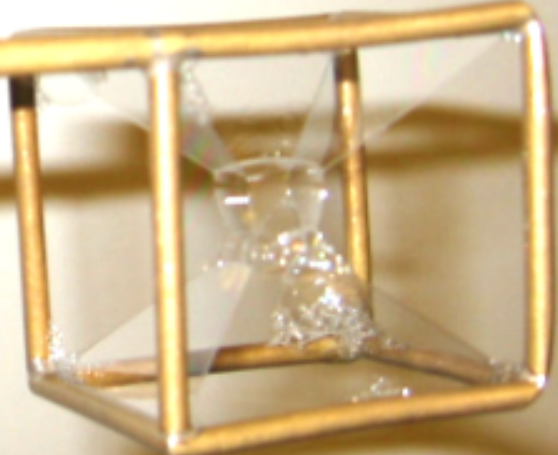
\includegraphics[width=0.8\textwidth]{Screenshot 2026-04-22 03.05.26.png}
    \caption*{Soap film \cite{highscalability_soapfilm}}
\end{figure}

\noindent \section*{Introduction}

Soap bubbles: a child’s game! Yet, behind them lies a wealth of theory and serious mathematics. Follow this document to glimpse the fascinating world of the mathematics hidden behind the laws of nature. Nature is well-designed: it economizes energy. Thus, soap forms its membrane in such a way as to use the least amount of space possible. This fascinating physical phenomenon is the concrete manifestation of a profound mathematical challenge: The Steiner Problem. As Frank Morgan describes in \cite{morgan1994soap}: \textit{“We prove existence and regularity for 'soap bubbles' in $\mathbb{R}^2$ and in surfaces, i.e., the least-perimeter way to enclose and separate regions of prescribed area. They consist of constant-curvature arcs meeting in threes at 120 degrees. If one prescribes the combinatorial type too, then the arcs may bump up against each other.”} This physical principle, where surface tension dictates a specific geometric regularity, serves as the gateway to our mathematical study. This project investigates the Steiner Problem within the modern framework of Analysis in Metric Spaces. \newline

Following the roadmap provided by \cite{ambrosio2004topics}, we decompose the study into three distinct phases:     

\paragraph{\hyperref[sec:param]{1. The Parametric Approach.}}
We first investigate the existence of a curve $\gamma$ of minimal length connecting two points $P$ and $Q$. Using the total variation and the metric derivative, we show that the Arzelà-Ascoli Theorem provides a solution in locally compact spaces, provided the curves are reparametrized by arc-length to ensure equicontinuity.

\paragraph{\hyperref[sec:nonparam]{2. Non-Parametric Formulation and Equivalence.}}
We then shift to a set-theoretic perspective, seeking a compact connected set $K$ that minimizes the 1-dimensional Hausdorff measure $\mathcal{H}^1(K)$. A key technical step (Part 2 bis) is to establish the equivalence between the length of a curve and the $\mathcal{H}^1$ measure of its image, utilizing the lower semicontinuity of the integral (Prop. 1.3.2) \cite{ambrosio2004topics}.
\paragraph{\hyperref[sec:steiner]{3. The Steiner Problem.}}
Finally, we extend the problem to $n$ points. We analyze the properties of Steiner trees, specifically the $120^\circ$ junction condition and the stability of connectedness under convergence. This section demonstrates how the Hausdorff distance and Hausdorff measure work together to guarantee the existence of a global minimum in abstract settings.

%%%%%%%%%%%%%%%%%%%%%%%%%%%%%%%%%%%%%%%%%%%%%%%%%%%%%%%%%%%%%%%%

\section{The Parametric Approach} \label{sec:param}

The first step in our study is to analyze the "shortest path" problem between two points $x, y$ in a metric space $(E, d)$ through the lens of continuous mappings. We define a curve as a continuous function $\gamma: [a, b] \to E$ such that $\gamma(a) = x$ and $\gamma(b) = y$. The goal of this section is to prove the goedesic problem : 

$$
    \min \{\ lengh(\gamma) : \gamma \ connects \ x \ to \ y \}
$$

\subsection{Length of Curves and Metric Derivative}

To quantify the cost of a path, we must first define its length. In a general metric space, we cannot rely on the classical Euclidean integral of the velocity vector. Instead, we use the {total variation as a universal definition.

\begin{definition}[Total Variation]
The length (or variation) of a curve $\gamma: [a, b] \to E$ is defined as:
\begin{equation}
    Var(\gamma)=Var_a^b(\gamma)=L(\gamma) = \sup \left\{ \sum_{i=0}^{n-1} d(\gamma(t_i), \gamma(t_{i+1})) : a = t_0 < t_1 < \dots < t_n = b \right\}
\end{equation}
where the supremum is taken over all possible finite partitions of the interval $[a, b]$. A curve is said to be \textbf{rectifiable} if $L(\gamma) < \infty$.
\end{definition}

While the total variation is general, it is difficult to manipulate in optimization problems. We therefore restrict our study to Lipschitz curves, which satisfy $d(\gamma(t), \gamma(s)) \leq L |t-s|$. 

Then the parametric problem reduces to :
\begin{equation}
    \min \{ L(\gamma) : \gamma \in Lip([a,b],E), \ \gamma(a)=x, \ \gamma(b)=y \}
\end{equation}

For such curves, as discussed in \cite{ambrosio2004topics}, we can introduce the metric derivative:

\begin{definition}[Metric Derivative]
For a Lipschitz curve $\gamma$, the metric derivative $|\dot{\gamma}|(t)$ exists for almost every $t \in [a, b]$ and is given by:
$$
    |\dot{\gamma}|(t) = \lim_{h \to 0} \frac{d(\gamma(t+h), \gamma(t))}{|h|}
$$
Furthermore, the length can be computed using the integral formula: $L(\gamma) = \int_a^b |\dot{\gamma}|(t) \, dt$.
\end{definition}

\begin{definition}[Path Integral] \cite{UE_analyse_complexe}
    Let D be a domain in the complex plane $\mathbb{C}$, and let C be a curve parametrized by the path: $\gamma : [a,b] \to \mathbb{C}$, $t \mapsto \gamma(t)$ such that $\gamma'(t)$ exists and is continuous. Let f be a continuous complex function defined on D: $f : D \to \mathbb{C}$, $\gamma \mapsto f(\gamma)$. The integral of f along the curve C is defined by
    $$
    \int_C f(z)\, dz = \int_a^b f(\gamma(t)) \cdot \gamma'(t)\, dt  
    $$
\end{definition}


\subsection{Existence of Geodesics}

The central problem of this section is to prove the existence of a geodesic, i.e., a curve $\gamma$ such that $L(\gamma) = \inf \{ L(\sigma) : \sigma \text{ connects } x \text{ to } y \}$ :

 \cite{Research} A geodesic represents the shortest path between two points on a given surface, with its specific nature differing between Euclidean and non-Euclidean geometries. In Euclidean geometry, a geodesic is a straight line, while in non-Euclidean contexts, such as Riemannian geometry, it is typically represented as a segment of a great circle, showcasing a curved trajectory. \\

Geodesics on simple spaces have essential properties in differential geometry:

\begin{itemize}
    \item Locally length-minimizing curve.

    \item Local uniqueness given point and tangent. 
    
    \item Zero geodesic curvature: $$\kappa_g = 0$$ Geodesic curvature measures how much a curve bends within the surface it lies on, and a geodesic is a curve with zero geodesic curvature, meaning it follows the straightest possible path on that surface.
    
    \item 
    The geodesic equation governs the path of geodesics in a Riemannian manifold: where $$\Gamma^\lambda_{\mu\nu}$$ are the Christoffel symbols of the second kind.This nonlinear second-order ODE system describes curves with zero geodesic curvature. The first term $$\frac{d^2 x^\lambda}{dt^2}$$ represents the coordinate acceleration, while the second term encodes how the manifold's geometry "pulls" the curve via its connection coefficients. Solutions to this equation are precisely the geodesics.
\end{itemize}

\begin{center}
    \textbf{Examples of geodesics on simple spaces}
\end{center} 

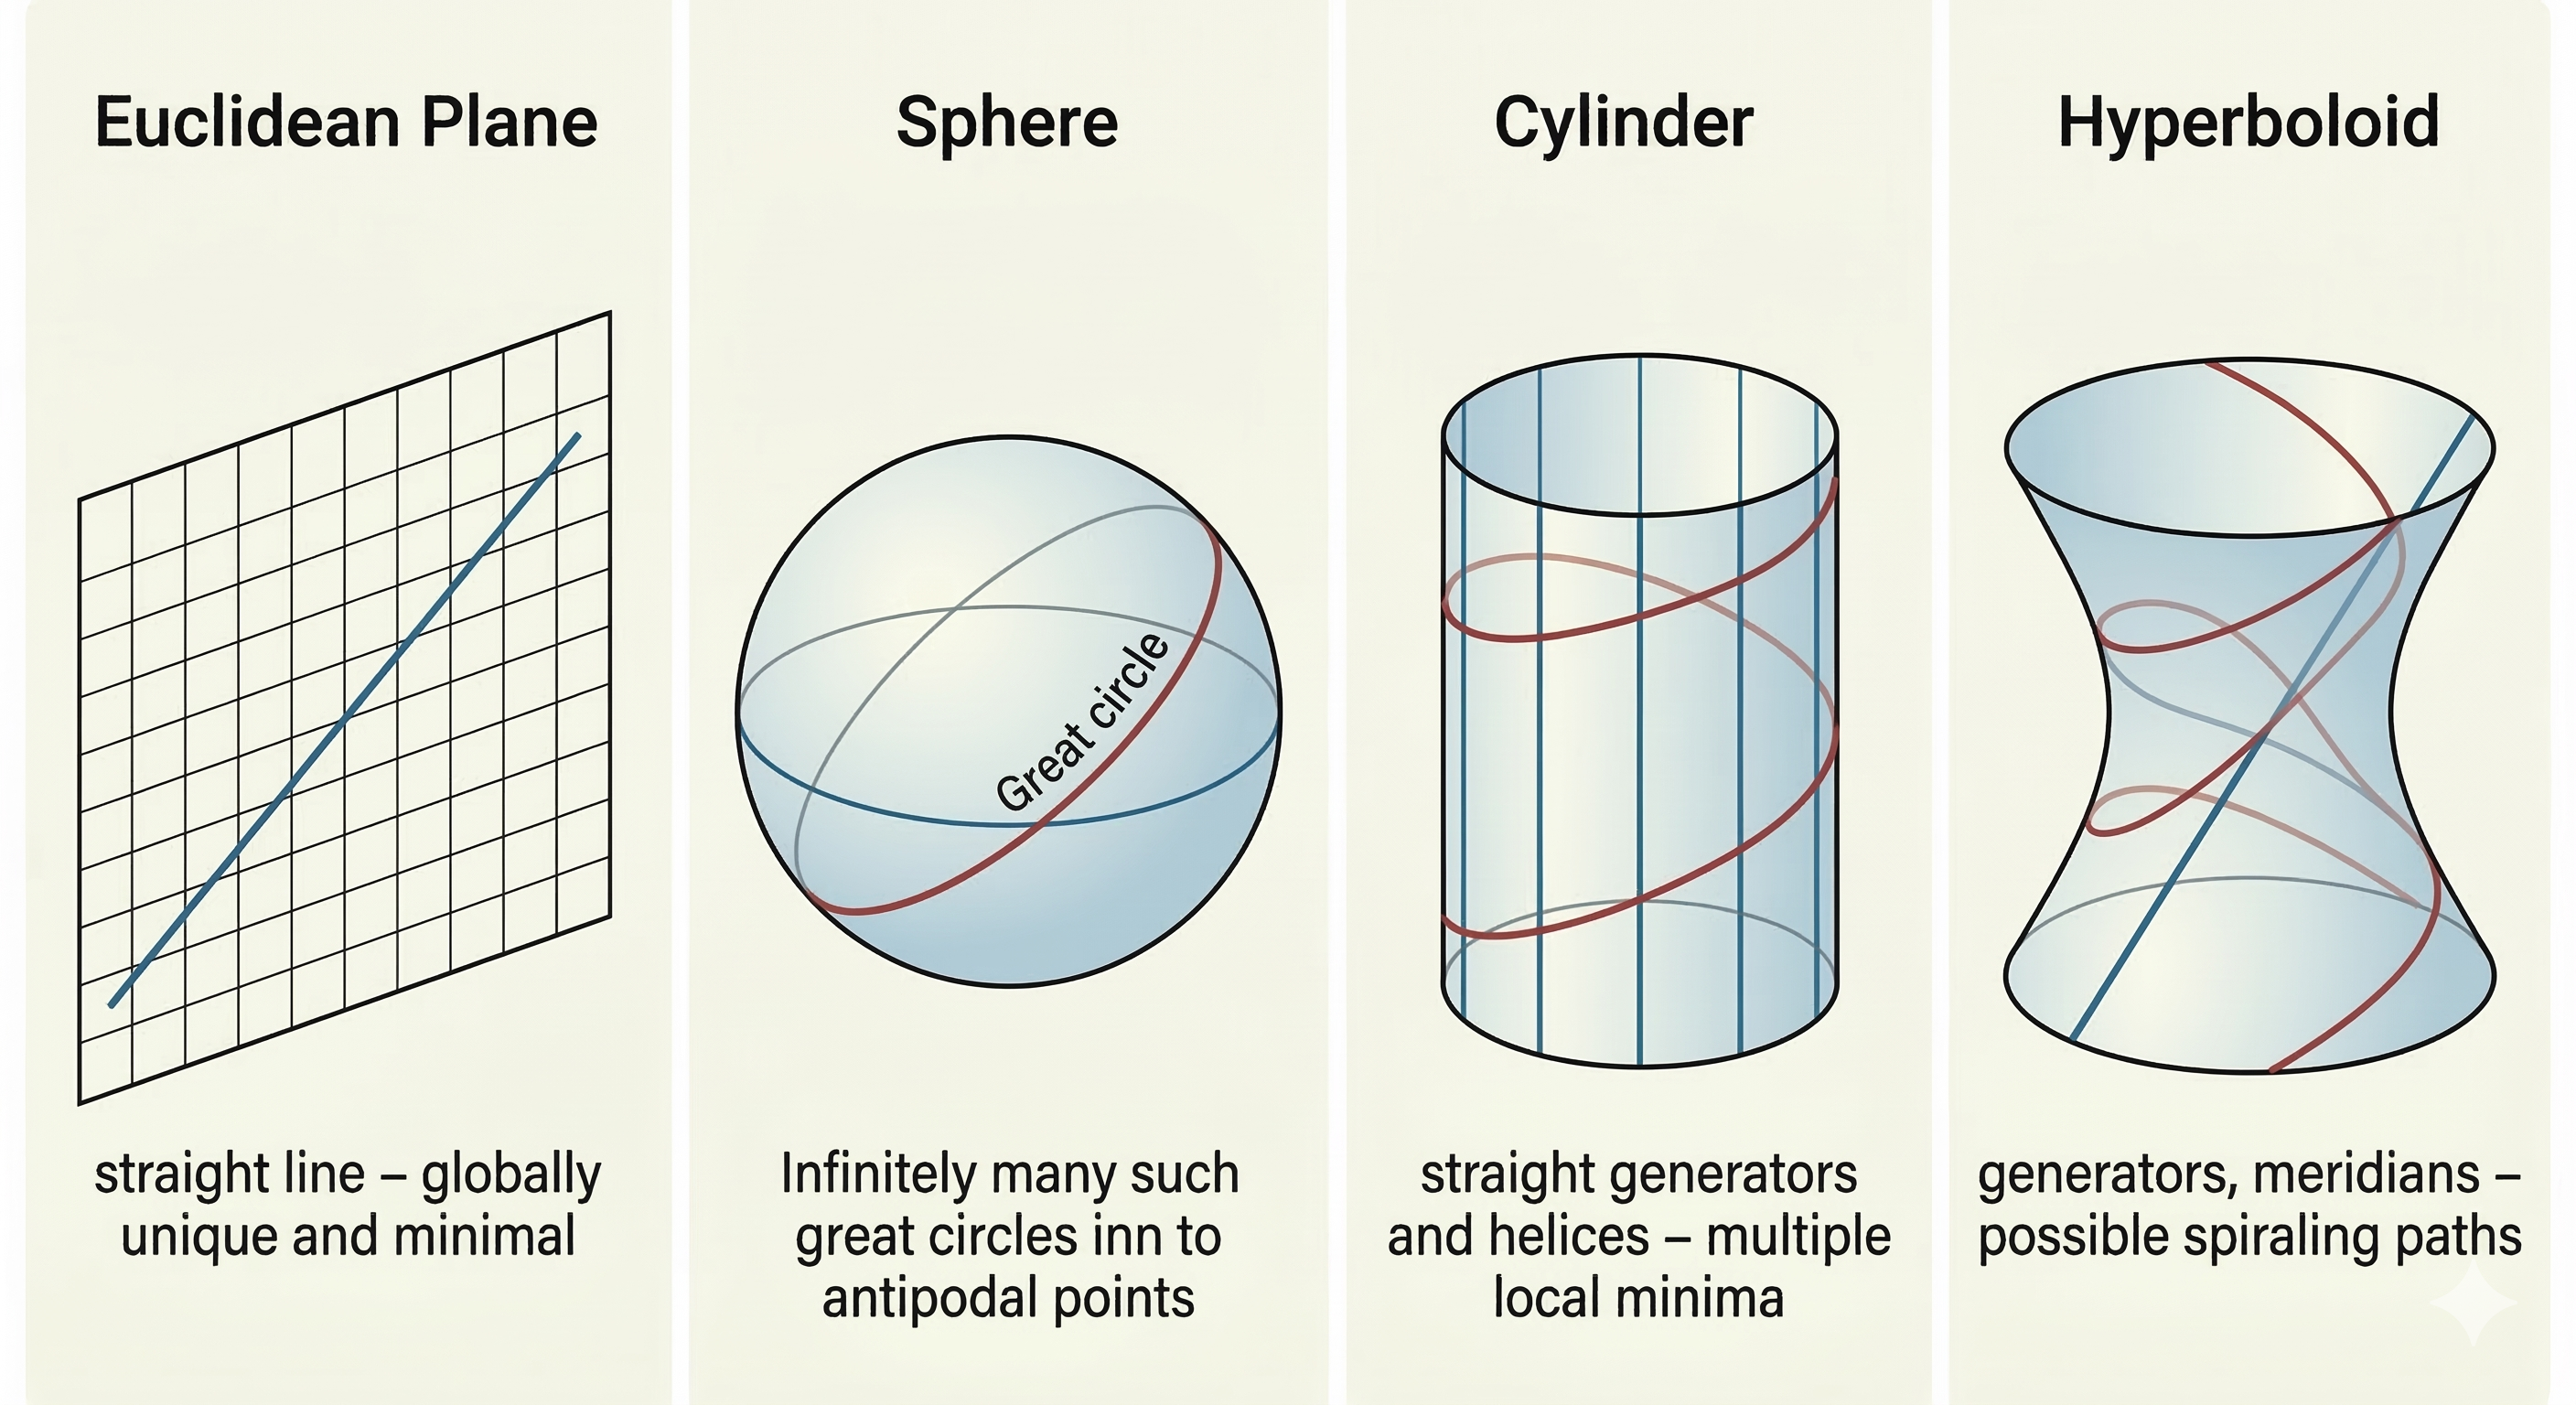
\includegraphics[width=0.9\textwidth]{geodesics.png}

The main difficulty in applying the direct method of the calculus of variations is that a minimizing sequence of curves may have "wild" parametrizations (e.g., stopping for a long time or moving extremely fast), which prevents the sequence from being equicontinuous. To solve this, we use the arc-length reparametrization:

\begin{theorem}[Reparametrization] \cite{ambrosio2004topics}
    Suppose that $\gamma \in \mathrm{Lip}([a,b],E)$, and let $L = \mathrm{Var}(\gamma)$ be its total variation. Then there exists a Lipschitz curve $\dot{\gamma} : [0,L] \mapsto E$ such that $|\dot{\tilde{\gamma}}|(t) = 1$ almost everywhere in $[0,L]$ and $ \dot\gamma([0,L]) = \gamma([a,b])$.
\end{theorem}

\begin{proof}
    Without loosing generality, we can assume that a=0. If $l(t)=Var^t_{0}(\gamma)$, we define : 
    $$
    h(t)=\inf \{ s \in [0,b] : l(s)=t \}, t \in [0,L],
    $$
    and observe that $h(0)=0$, h is nondecreasing and $h(L) \leq b$. Moreover, 
    \begin{equation}
    l(h(t))=t \quad and \quad \gamma(s)=\gamma(h(l(s))) \tag{1}
    \end{equation}
    for $t \in [0,L]$ and $s \in [0,b]$. Indeed, the first equality is immediate and for the second, we observe that : $h(l(s)) \leqslant s$ and
    $$
    d\big(\gamma(h(l(s))), \gamma(s)\big) \leqslant \mathrm{Var}^{s}_{h(l(s))}(\gamma)
    $$
    $$
    = l(s) - l(h(l(s)))
    $$
    $$
    = l(s) - l(s) = 0.
    $$
    Then we define
    $$
    \tilde{\gamma}(t) := \gamma(h(t)), \quad t \in [0, L],
    $$
    and claim that $\tilde{\gamma}$ has all of the required properties (we remark that $h(t)$ need not be continuous). Observe that the identity

    \begin{equation}
    \mathrm{Var}_0^t(\tilde{\gamma}) = t \quad \forall t \in [0, L] \tag{2}
    \end{equation}

    is a consequence of the definition of $h(t)$. Indeed, if $0 \leqslant t_1 \leqslant \cdots \leqslant t_n \leqslant t$, letting $s_i = h(t_i)$ we have

    \begin{align*}
        \sum_{i=1}^{n-1} d\!\left(\tilde{\gamma}(t_{i+1}),\tilde{\gamma}(t_i)\right)
        &= \sum_{i=1}^{n-1} d\!\left(\gamma(s_{i+1}), \gamma(s_i)\right) \\
        &\leqslant \mathrm{Var}_0^{s_n}(\gamma) = l(s_n) = t_n \leqslant t.
    \end{align*}

    Taking the supremum over all partitions yields

    \begin{equation}
        \mathrm{Var}_0^t(\tilde{\gamma}) \leqslant t. \tag{3}
    \end{equation}

    On the other hand, for $t \in [0, L]$ and $\varepsilon > 0$, we can find numbers
    $0 = s_1 \leqslant \cdots \leqslant s_n = h(t)$ such that

    \[
        l(h(t)) \leqslant \varepsilon + \sum_{i=1}^{n-1} d\!\left(\gamma(s_{i+1}), \gamma(s_i)\right).
    \]

    Using (1), we obtain

    \begin{align*}
        t &\leqslant \varepsilon + \sum_{i=1}^{n-1} d\!\left(\gamma(h(l(s_{i+1}))), \gamma(h(l(s_i)))\right) \\
          &= \varepsilon + \sum_{i=1}^{n-1} d\!\left(\tilde{\gamma}(l(s_{i+1})), \gamma(l(s_i))\right) \\
          &\leqslant \varepsilon + \mathrm{Var}_{l(s_1)}^{l(s_n)}(\tilde{\gamma}) \\
          &= \varepsilon + \mathrm{Var}_0^{l(h(t))}(\tilde{\gamma}) \\
          &= \varepsilon + \mathrm{Var}_0^t(\tilde{\gamma}),
    \end{align*}

    which, combined with (3), yields (2) since $\varepsilon > 0$ was arbitrary.
    In particular, from (2), it follows that $\tilde{\gamma}$ is 1-Lipschitz.

    Finally, as long as $\gamma$ is Lipschitz, one obtains

    \[
        t = \mathrm{Var}_0^t(\tilde{\gamma}) = \int_0^t |\dot{\tilde{\gamma}}|(\tau)\, \mathrm{d}\tau
        \quad \forall t \in [0, 1],
    \] 
    
    and, differentiating with respect to $t$, we have $|\dot{\tilde{\gamma}}|(t) = 1$ for almost
    every $t$. Finally, the equality $\gamma([a, b]) = \tilde{\gamma}([0, L])$ follows easily from
    (1). \qed \hfill\myqedsymbol

\end{proof}

\begin{theorem}[Ascoli-Arzelà Revisited]
    Let $K$ and $E$ be two metric spaces with $K$ compact, and let $\{\gamma_m\}$ be a sequence of continuous functions from $K$ into $E$ such that:
    \begin{itemize}
        \item $\{\gamma_m\}$ is equicontinuous;
        \item There exists a compact set $C \subseteq E$ such that for every $\delta$-neighborhood $C_\delta$ of $C$, we have $\gamma_m(K) \subseteq C_\delta$ provided that $m$ is sufficiently large.
    \end{itemize}
   Under the above assumptions, there exists a continuous function $\gamma : K \to C$ and a subsequence $\{m_k\}$ such that $\{\gamma_{m_k}\}$ converges uniformly to $\gamma$ on $K$.
\end{theorem}

\begin{theorem}
    Suppose that $E$ i s a compact metric space. Then the minimum problem (1.2) admits a solution, provided that the class of Lipschitz curves connecting x and y is not empty.
\end{theorem}

\begin{proof}
    Let $L$ be the value of the infimum for the problem, and let $\{\gamma_n\}$ 
    be a minimizing sequence, that is,
    \[
        \gamma_n : [a,b] \to E, \quad \gamma_n(a) = x, \quad \gamma_n(b) = y, 
        \quad \lim_{n \to \infty} L_n = L,
    \]
    where $L_n = \mathrm{Var}(\gamma_n)$. Without loss of generality we assume 
    that $L > 0$ (otherwise $x = y$ and the problem is trivial) and that 
    $L_n \leqslant L + 1$. According to the reparametrization theorem 
    (Theorem 1.4), we can assume that $\gamma_n$ is defined on $[0, L_n]$ 
    with $|\dot{\gamma}_n| = 1$ almost everywhere. By a further linear change 
    of variable (namely, $t \mapsto tL/L_n$), we can assume that each 
    $\gamma_n$ is defined over $[0, L]$ and $|\dot{\gamma}_n| = L_n/L$.

    In particular, we have $\mathrm{Lip}(\gamma_n) \leqslant (L+1)/L$; hence 
    the sequence $\{\gamma_n\}$ is equicontinuous. Since $E$ was supposed to 
    be compact, the Ascoli–Arzelà theorem infers the existence of a 
    subsequence $\{\gamma_{n_k}\}$ which is uniformly convergent on $[0, L]$ 
    to a Lipschitz function $\gamma$.

    Observe that, for every fixed partition $a \leqslant t_1 \leqslant \cdots 
    \leqslant t_n \leqslant b$, each summation in (1.1) (regarded as a 
    functional on $\mathrm{Lip}([0,L], E)$) is continuous with respect to the 
    uniform convergence. As a consequence, the functional
    \[
        \mathrm{Var} : \mathrm{Lip}([0, L], E) \to \mathbb{R}
    \]
    (as the supremum of a family of continuous functionals) is lower 
    semicontinuous with respect to the uniform convergence. Therefore, since 
    in our case $\{\gamma_{n_k}\}$ converges uniformly to $\gamma$, we obtain
    \[
        L \leqslant \mathrm{Var}(\gamma) \leqslant \liminf_{k \to \infty} 
        \mathrm{Var}(\gamma_{n_k}) = \liminf_{k \to \infty} L_{n_k} = L,
    \]
    and hence $\gamma$ is a minimizer for (1.2).
\end{proof}

%%%%%%%%%%%%%%%%%%%%%%%%%%%%%%%%%%%%%%%%%%%%%%%%%%%%%%%%%%%%%%%%

\section{Tools to prove the equivalence between the parametric and the intinsic Problem} \label{sec:nonparam}

\subsection{Properties of the Haudorff measures}

In this subsection, we focus on some properties and definitions that are usefull for us on Hausdorff measures, for the Steiner problem, we focus on the 1-dimentional Hausdorff measure.

\begin{definition}[Unidimentional Hausdorff measure]
    $\mathcal{H}^1$ denotes the unidimentionnal Hausdorff measure, defined for every subset $A \subseteq E$ as $$\mathcal{H}^1(A) = \lim\limits_{\delta \rightarrow 0^+} \mathcal{H}_\delta^1(A)$$ where $\mathcal{H}_\delta^1$ is given by $$\mathcal{H}_\delta^1(A) = \inf \{ \sum_{i=1}^{\infty} diam(A_i) : \ A \subseteq \bigcup A_i, \ diam(A_i) \leq \delta \}$$ 
\end{definition}

\begin{lemma}
    If $\gamma : [a, b] \to E$ is continuous, then \[ \mathcal{H}^1(\gamma([a,b])) \ge dist(\gamma(a),\gamma(b)) \]
\end{lemma}

\begin{proof}
    Define the auxiliary function $\varphi(x) := \mathrm{dist}(x, \gamma(a))$. 
    Then $\varphi : E \to \mathbb{R}$ is 1-Lipschitz, and hence
    \[
        \mathcal{H}^1\!\left(\varphi(\gamma([a, b]))\right) \leqslant 
        \mathcal{H}^1\!\left(\gamma([a, b])\right).
    \]
    On the other hand, since $\mathcal{H}^1$ coincides on $\mathbb{R}$ with the 
    outer Lebesgue measure, and $\varphi(\gamma([a, b]))$ is an interval of the 
    form $[0, \sigma]$, we obtain
    \begin{align*}
        \mathcal{H}^1\!\left(\varphi(\gamma([a, b]))\right) 
        &= \sup_{t \in [a, b]} \varphi(\gamma(t)) \\
        &= \sup_{t \in [a, b]} \mathrm{dist}\!\left(\gamma(t), \gamma(a)\right) \\
        &\geqslant \mathrm{dist}\!\left(\gamma(a), \gamma(b)\right),
    \end{align*}
    and the proof is completed.
\end{proof}

\begin{theorem}
    Suppose that $\gamma : [a, b] \to E$ is a Lipschitz curve and let $\Gamma = \gamma([a, b])$ be its range. Then:

    \begin{equation}
        \mathcal{H}^1(\Gamma) \leqslant \text{Var}(\gamma)
    \end{equation}
    and equality holds if $\gamma$ is injective.
\end{theorem}

\begin{proof}
    Due to the reparametrization theorem, it is not restrictive to assume that 
    $|\dot{\gamma}| = 1$, $a = 0$, and $b = \mathrm{Var}(\gamma)$. Given 
    $\delta > 0$, choose $n \in \mathbb{N}$ such that $\mathrm{Var}(\gamma)/n < \delta$, 
    and let $h := \mathrm{Var}(\gamma)/n$ and $J_i := [ih, (i+1)h]$, 
    $i = 0, \ldots, n-1$.

    Since $\gamma$ is 1-Lipschitz, we have $\mathrm{diam}(\gamma(J_i)) \leqslant 
    \mathrm{diam}(J_i) < \delta$; hence
    \[
        \mathcal{H}^1_\delta(\Gamma) \leqslant \sum_{i=0}^{n-1} \mathrm{diam}(J_i) 
        = \mathrm{Var}(\gamma),
    \]
    and (2.1) follows since $\delta > 0$ was arbitrary.

    Now suppose that $\gamma$ is injective, and choose $a \leqslant t_0 < \cdots 
    < t_n \leqslant b$. We have from Lemma 2.2 that
    \begin{align*}
        \sum_{i=0}^{n-1} \mathrm{dist}\!\left(\gamma(t_{i+1}), \gamma(t_i)\right) 
        &\leqslant \sum_{i=0}^{n-1} \mathcal{H}^1\!\left(\gamma([t_i, t_{i+1}])\right) \\
        &\leqslant \mathcal{H}^1\!\left(\gamma([a, b])\right)
    \end{align*}
    (the last inequality relies on the injectivity of $\gamma$ and the additivity 
    of the Hausdorff measure). Since the partition $\{t_i\}$ was arbitrary, we 
    deduce $\mathrm{Var}(\gamma) \leqslant \mathcal{H}^1\!\left(\gamma([a, b])\right)$, 
    and hence equality holds in (2.1).
\end{proof}

\begin{remark}
    We see that the Hausdorff measure comparable the total variation of a curve, the points of non-injectivity being the cause of the inequality (2.1).
\end{remark}

\begin{theorem}[Hausdorff and Radon measures]
    Let $\mu$ be a positive and locally-finite measure in $E$. Then, for any $t \in (0, +\infty)$ and any Borel set $B \subseteq E$, the following implications hold:
    \begin{align}
    \overline{\Theta}_1(\mu, x) \ge t \quad \forall x \in B \quad &\Longrightarrow \quad \mu(B) \ge t \, \mathcal{S}^1(B) \ge t \, \mathcal{H}^1(B).  \\
    \overline{\Theta}_1(\mu, x) \le t \quad \forall x \in B \quad &\Longrightarrow \quad \mu(B) \le 2t \, \mathcal{H}^1(B). 
    \end{align}
\end{theorem}

\begin{remark}
    \begin{itemize}
        \item [(i)] $\overline{\Theta}_1(\mu, x)$ is the measure of spherical density define by : \[ \overline{\Theta}_1(\mu, x) = \limsup_{r \to 0^+} \frac{\mu(B(x,r))}{r} \]
        \item[(ii)] $\mathcal{S}^1$ is the 1-dimentional spherical Hausdorff measure.
    \end{itemize}
\end{remark}



\subsection{Geometry of 1-dimensional sets}

\begin{lemma}[Density lower bound]
    If $C \subseteq E$ is connected and $0<r<diam(C)/2$, then $$\mathcal{H}^1(C \cap B(x,r)) \geq r, \ \forall x \in C$$
\end{lemma}

\begin{proof}
    Choose $x \in C$ and define $\varphi(y) := \mathrm{dist}(x, y)$, $y \in E$. Observe 
    that $\varphi$ is 1-Lipschitz, and hence
    \[
        \mathcal{H}^1\!\left(\varphi(C \cap B_r(x))\right) \leqslant \mathcal{H}^1\!\left(C \cap B_r(x)\right).
    \]
    On the other hand, since $\mathcal{H}^1$ on $\mathbb{R}$ is an outer Lebesgue measure and 
    $\varphi(C \cap B_r(x))$ is an interval of the form $[0, a]$, we obtain
    \begin{align*}
        \mathcal{H}^1\!\left(\varphi(C \cap B_r(x))\right) 
            &= \sup_{y,z \in C \cap B_r(x)} |\mathrm{dist}(x,y) - \mathrm{dist}(x,z)| \\
            &= \sup_{y \in C \cap B_r(x)} \mathrm{dist}(x, y) \geqslant r
    \end{align*}
    (the last inequality follows easily from the fact that $C$ is connected).
\end{proof}

\begin{definition}[$\varepsilon$-connectedness]
    Let $C \subseteq E$ and $x, y \in C$. We say that $x$ and $y$ are 
    $\varepsilon$-connected in $C$ if there exist $x_1, \ldots, x_n \in C$ such 
    that $x_1 = x$, $x_n = y$, and $\mathrm{dist}(x_i, x_{i+1}) < \varepsilon$. 
    In this case, we say that $\{x_1, \ldots, x_n\}$ is an $\varepsilon$-chain 
    in $C$ joining $x$ and $y$.
\end{definition}

\begin{theorem}[Isometric embedding]
    Suppose that $E$ is a separable metric space, then there exists an isometry $J : E \to l^\infty$.
\end{theorem}

\begin{proof}
    Let $\{x_n\}_{n \geqslant 1} \subseteq E$ be a dense sequence, and define
    \begin{align*}
        J(x)_n &:= \mathrm{dist}(x, x_n) - \mathrm{dist}(x_1, x_n), \quad n = 1, 2, \ldots, \\
        J(x) &:= \{J(x)_n\}_{n=1}^{\infty}.
    \end{align*}
    Observe that from the triangle inequality one has
    \begin{align*}
        \|J(x)\|_{\ell^\infty} &= \sup_{n \geqslant 1} \left| \mathrm{dist}(x, x_n) 
        - \mathrm{dist}(x_1, x_n) \right| \\
        &\leqslant \mathrm{dist}(x, x_1) < +\infty;
    \end{align*}
    hence $J(x) \in \ell^\infty$ and $J : E \to \ell^\infty$ is well defined. 
    In a similar fashion, for every pair $x, y \in E$ one easily obtains
    \begin{equation}
        \|J(x) - J(y)\|_{\ell^\infty} \leqslant \mathrm{dist}(x, y).
    \end{equation}
    Moreover, for every $\varepsilon > 0$ and every pair $x, y \in E$ there exists 
    $n$ such that $\mathrm{dist}(x, x_n) < \varepsilon$, and hence
    \begin{align*}
        \|J(x) - J(y)\|_{\ell^\infty} 
        &\geqslant \left| \left(\mathrm{dist}(x, x_n) - \mathrm{dist}(x_1, x_n)\right) 
        - \left(\mathrm{dist}(y, x_n) - \mathrm{dist}(x_1, x_n)\right) \right| \\
        &= \left| \mathrm{dist}(x, x_n) - \mathrm{dist}(y, x_n) \right| \\
        &= \left| \mathrm{dist}(x, x_n) - \mathrm{dist}(x, y) + \mathrm{dist}(x, y) 
        - \mathrm{dist}(y, x_n) \right| \\
        &\geqslant \mathrm{dist}(x, y) - \left| \mathrm{dist}(x, y) 
        - \mathrm{dist}(y, x_n) \right| - \mathrm{dist}(x, x_n) \\
        &\geqslant \mathrm{dist}(x, y) - 2\varepsilon.
    \end{align*}
    Thus, from the arbitrariness of $\varepsilon > 0$, one deduces that equality 
    holds in (2.4). Therefore, $J$ is an isometry and the proof is completed.
\end{proof}

\begin{theorem}[First rectifiability theorem]
    If $E$ is complete and $C \subseteq E$ is a closed connected set such 
    that $\mathcal{H}^1(C) < +\infty$, then $C$ is compact and connected 
    by injective rectifiable curves.
\end{theorem}

\begin{proof}
    Choose $x_0 \in C$ and $\varepsilon > 0$ such that $\varepsilon < \mathrm{diam}(C)$ 
    (if $\mathrm{diam}(C) = 0$ then $C = \{x_0\}$ and the statement is trivial). 
    For $n \geqslant 1$, inductively choose
    \[
        x_n \in C \setminus \bigcup_{i=0}^{n-1} B_{\varepsilon}(x_i),
    \]
    stopping the process as soon as $\bigcup_{i=0}^{n-1} B_{\varepsilon}(x_i)$ covers 
    all of $C$. We claim that the process terminates after a finite number of steps. 
    Indeed, the sets $C \cap B_{\varepsilon/2}(x_i)$ are pairwise disjoint and are a 
    positive distance apart. Hence, if the process is not yet terminated after $n$ 
    steps, we have
    \[
        \mathcal{H}^1(C) \geqslant \sum_{i=0}^{n-1} \mathcal{H}^1\!\left(C \cap 
        B_{\varepsilon/2}(x_i)\right) \geqslant n \frac{\varepsilon}{2},
    \]
    where the last inequality follows from density lower bound theorem (Lemma 2.7) Since $\mathcal{H}^1(C)$ 
    was assumed to be finite, we have proved that $n$ cannot grow arbitrarily 
    large; hence the process is terminated after finitely many steps. The above 
    construction shows that $C$ is totally bounded, and hence it is a compact set.

    Since the statement of the theorem is invariant under isometries, due to 
    isometric embedding theorem (Theorem 2.9) we can assume, without loss of generality, that $E = \ell^\infty$.

    For $\varepsilon > 0$ and $x \in C$, define
    \[
        C'_x := \{y \in C \mid x \text{ and } y \text{ are } \varepsilon\text{-connected in } C\}.
    \]
    It is easy to see that $C'_x$ is open and closed in $C$; hence $C'_x = C$ since 
    $C$ is connected. Therefore, for every $\varepsilon > 0$ and every $y \in C$ we 
    can find an $\varepsilon$-chain $\{x_1, \ldots, x_n\} \subseteq C$ joining $x$ 
    and $y$. Moreover, reducing the chain, if necessary, we can assume that
    \[
        \mathrm{dist}(x_i, x_j) \geqslant \varepsilon \quad \text{whenever } |i - j| > 1.
    \]
    Observe that the above inequality implies that any two distinct balls 
    $\{B_{\varepsilon/2}(x_i)\}$ and $\{B_{\varepsilon/2}(x_j)\}$ are a positive 
    distance apart, provided that $i$ and $j$ are both odd or both even. Therefore, 
    we obtain
    \[
        \mathcal{H}^1(C) \geqslant \mathcal{H}^1\!\left(C \cap \bigcup_{i \text{ odd}} 
        B_{\varepsilon/2}(x_i)\right) = \sum_{i \text{ odd}} \mathcal{H}^1\!\left(C \cap 
        B_{\varepsilon/2}(x_i)\right).
    \]
    If $\varepsilon < \mathrm{diam}(C)$, from density lower bound (Lemma 2.7) and the last inequality we 
    obtain
    \[
        \mathcal{H}^1(C) \geqslant \sum_{i \text{ odd}} \frac{\varepsilon}{2}.
    \]
    Adding the above inequality and the analogous one concerning the even subscripts, 
    we obtain
    \[
        2\, \mathcal{H}^1(C) \geqslant n \frac{\varepsilon}{2},
    \]
    which provides an upper bound for the size $n$ of the $\varepsilon$-chain in 
    terms of $\varepsilon$ and $\mathcal{H}^1(C)$.

    All in all, given $x, y \in C$ and $\varepsilon > 0$ with $\varepsilon < 
    \mathrm{diam}(C)$, we can find an $\varepsilon$-chain $\{x_i\}_{i=1}^n \subseteq C$ 
    which connects $x$ and $y$, and the size $n$ of the chain satisfies 
    $n \leqslant 4\mathcal{H}^1(C)/\varepsilon$. The assumption that $E = \ell^\infty$ 
    provides us with a vector space structure, and hence there exists a Lipschitz 
    curve $\gamma_\varepsilon : [0, L] \to \ell^\infty$, where $L = 4\mathcal{H}^1(C)$, 
    characterized as follows:
    \begin{itemize}
        \item there exists a partition $0 = t_1 < t_2 < \cdots < t_n \leqslant L$ 
              such that $t_{i+1} - t_i = \mathrm{dist}(x_{i+1}, x_i) < \varepsilon$;
        \item $\gamma_\varepsilon(s) = x_i + (s - t_i)(x_{i+1} - x_i)/(t_{i+1} - t_i)$ 
              if $s \in [t_i, t_{i+1}]$;
        \item $\gamma_\varepsilon(s) = x_n = y$ if $s \in [t_n, L]$;
        \item $\gamma_\varepsilon$ is 1-Lipschitz;
        \item $\gamma_\varepsilon(s)$ belongs to the $\varepsilon$-neighborhood of 
              $C$ (in $\ell^\infty$) for all $s \in [0, L]$.
    \end{itemize}
    Since $C$ is compact and the family $\{\gamma_\varepsilon\}$ is equicontinuous, 
    we can apply Ascoli-Arzelà revisited with $K := [0, L]$, thus obtaining the existence of 
    a Lipschitz function $\gamma : [0, L] \to C$ joining $x$ and $y$.

    Finally, the existence of an injective Lipschitz curve joining $x$ and $y$ in 
    $C$ follows from the geodesic existence theorem (Theoreme 1.6), applied with $C$ (which is compact) in place 
    of $E$.
\end{proof}

\begin{theorem}[Second rectifiability theorem]
    If $E$ is complete, $C \subseteq E$ is closed and connected, and 
    $\mathcal{H}^1(C) < +\infty$, then there exist countably many Lipschitz 
    curves $\gamma_i : [0, 1] \mapsto C$ such that
    \[
        \mathcal{H}^1\!\left(C \setminus \bigcup_{i=1}^{\infty} \gamma_i([0,1])\right) = 0.
    \]
    In other words, $\mathcal{H}^1$-almost all of $C$ can be covered by a 
    countable family of Lipschitz curves.
\end{theorem}

\begin{proof}
    This theorem is admitted, it is used only for the theorem of existence for the intrinsic problem.
\end{proof}


%%%%%%%%%%%%%%%%%%%%%%%%%%%%%%%%%%%%%%%%%%%%%%%%%%%%%%%%%%%%%%%%

\section{The Steiner Problem} \label{sec:steiner}

To prove the existence of the existence of the intrinsic formulation 

\begin{equation}
     \min \{ \ \mathcal{H}^1(C) : \ C \ connected \ and \ closed, \ and \ C' \subseteq C \ \}
\end{equation}

where $C'$ is a closed nonempty subset of E, we use the direct method of calculus of variations, so we need to choose a metric space and we verify that its compact and lower semi-continuous to ensure that there is a minimizing sub-sequence.

We begin by defining the Hausdorff distance, which measures the distances between sets.

\begin{definition}[Hausdorff distance]
    Let $\mathcal{C}_E$ be the family of all nonempty closed subsets of the metric space $E$. For $C, D \in \mathcal{C}_E$, the Hausdorff distance $d_H(C, D)$ is defined as:$$d_H(C, D) := \min\{1, h(C, D)\}$$where $h(C, D) := \inf\{r \in [0, +\infty] \mid C \subseteq D_r \text{ and } D \subseteq C_r\}$, and $S_r$ denotes the $r$-neighborhood of $S$.
\end{definition}

\begin{proposition}
    The function $d_H$ is a metric on $\mathcal{C}_E$, called the Hausdorff distance.
\end{proposition}


\begin{proof}
    Choose $C, D, F \in \mathcal{C}_E$, and suppose that there exist $0 < r, r' \leqslant 1$ such that:
    \begin{equation*}
         C \subset F_r, \quad F \subset C_r, \quad F \subset D_{r'}, \quad D \subset F_{r'}. \tag{*}
    \end{equation*} It is easy to see that $C \subset D_{r+r'}$ and $D \subset C_{r+r'}$; hence$$d_H(C, D) \leqslant h(C, D) \leqslant r + r'.$$ Taking the infimum over all the pairs $r, r' \in (0, 1]$ satisfying $(*)$, we obtain
    \begin{equation*}
        d_H(C, D) \leqslant d_H(C, F) + d_H(F, D). \tag{**}
    \end{equation*}On the other hand, if no pair $r, r' \in (0, 1]$ simultaneously satisfy the four conditions $(*)$, then we necessarily have $\max\{h(C, F), h(F, D)\} \geqslant 1$, and $(**)$ is trivially satisfied. All in all, $d_H$ satisfies the triangle inequality.
    
    Now suppose that $d_H(C, D) = 0$. Then $C \subseteq \bigcap_\varepsilon D_\varepsilon = D$ since $D$ is closed, and hence $C \subseteq D$. By symmetry, $C = D$. Finally, the proof that $d_H(C, C) = 0$ is immediate.
\end{proof}

\begin{proposition}[Completeness]
    The metric space $(\mathcal{C}_E,d_H)$ is complete, provided that $E$ itself is complete.
\end{proposition}

\begin{proof}
    Suppose that $\{C_n\} \subseteq C_E$ is a Cauchy sequence with respect to $d_H$. Disregarding, if necessary, only a finite number of sets of the sequence, we may assume that $d_H(C_n, C_m) < 1$ for all $n$ and $m$, and hence that $d_H(C_n, C_m) = h(C_n, C_m)$.
    
    Due to the Cauchy property, there exists an increasing sequence of numbers $\{N_k\}$ such that
    
    $$h(C_n, C_m) = d_H(C_n, C_m) < 2^{-k} \quad \forall n, m \ge N_k.$$
    
    Choose $x_1 \in C_{N_1}$. Since $C_{N_1} \subset (C_{N_2})_{1/2}$, there exists $x_2 \in C_{N_2}$ such that $\text{dist}(x_1, x_2) < 1/2$. We can proceed inductively, choosing $x_k \in C_{N_k}$ such that $\text{dist}(x_k, x_{k+1}) < 2^{-k}$. Thus we obtain a Cauchy sequence $\{x_k\}$ which is convergent to some $x \in E$. Now define
    
    $$D_k := \overline{\bigcup_{j \ge k} C_{N_j}}$$
    
    and observe that $D_k$ is closed in $E$ and $x_j \in D_k$ if $j \ge k$. Therefore, the limit point $x$ belongs to every $D_k$. Letting $C := \bigcap_k D_k$, we see that $C$ is closed and nonempty, since $x \in C$. Observe that
    
    \begin{equation*}
        C \subset D_k \subset \overline{(C_{N_k})_{2^{-k}}} \subset (C_{N_k})_{2^{1-k}}. \tag{***}
    \end{equation*}
    
    On the other hand, for $j \ge k$ we have
    
    $$C_{N_k} \subset (C_{N_j})_{2^{-k}} \subseteq (D_j)_{2^{-k}},$$
    
    which implies that $C_{N_k} \subset (C)_{2^{1-k}}$. The last inequality combined with $(***)$ yields
    
    $$d_H(C_{N_k}, C) \le 2^{1-k}.$$
    
    Finally, we have for all $k$
    
    $$\begin{aligned} \limsup_{n \to \infty} d_H(C_n, C) &\le \limsup_{n \to \infty} d_H(C_n, C_{N_k}) + d_H(C_{N_k}, C) \\ &\le 2^{-k}; \end{aligned}$$
    
    hence $C_n$ converges to $C$ since $k$ was arbitrary.
\end{proof}


\begin{definition}[Kuratowski convergence]
    A sequence of closed sets $\{Cn\} \subseteq E$ is said to converge in the sence of Kuratowski to a closed set C if the following two conditions are satisfied : 
    \begin{itemize}
        \item[(i)] If $x = \lim_{k \to \infty} x_{n_k}$ for some subsequence 
        $\{x_{n_k}\}$ of a sequence $\{x_n\}$ such that $x_n \in C_n$, 
        then $x \in C$.
        \item[(ii)] If $x \in C$, then there exists a whole sequence $\{x_n\}$ 
        such that $x_n \in C_n$ and $x = \lim_{n \to \infty} x_n$.
    \end{itemize}
    We denote the above convergence by writing $C_n \xrightarrow{K} C$.
\end{definition}

\begin{theorem}[Blaschke]
    If the metric space $E$ is compact, then the space of its closed subsets $(\mathcal{C}_E, d_H)$ is also a compact metric space.
\end{theorem}

\begin{proof}
    Since $E$ is compact, it is complete and totally bounded. Since $\mathcal{C}_E$ is complete by the proposition 3.3, we have to show that $\mathcal{C}_E$ is totally bounded. Given $\epsilon > 0$, choose a finite subset $F \subset E$ whose $\epsilon$-neighborhood covers all of $E$ and let $\mathcal{F} \subset \mathcal{C}_E$ be the finite collection of all nonempty subset of $F$. It is easy to see that the $\epsilon$-neighborhood of $(\mathcal{F},d_H)$ covers all $\mathcal{C}_E$. Therefore, $\mathcal{C}_E$ is totally bounded, and hence it is compact.
\end{proof}

\begin{theorem}[Golab]
    Let $E$ be a complete metric space. Suppose that $\{C_n\} \subseteq \mathcal{C}_E$ is a sequence of connected closed sets such that $C_n \xrightarrow{d_H} C$. Then $C$ is connected and:$$\mathcal{H}^1(C) \leqslant \liminf_{n \to \infty} \mathcal{H}^1(C_n)$$
\end{theorem}

\begin{proof}

Without loss of generality, we can suppose that $L :=
\lim_{n \to \infty} \mathcal{H}^1(C_n)$ exists and is finite, and that $\mathcal{H}^1(C_n) < L + 1$ for all $n$.
Then, by the first rectifiability theorem, we can also assume that each $C_n$ is compact.
Firstly, it is clear that $C$ is connected (this follows easily from $C_n \xrightarrow{H} C$
and from the fact that each $C_n$ is connected).

\indent Let us reduce to the case where $E$ is compact. Define
\[
    \tilde{E} := \overline{\bigcup_{n=1}^{\infty} C_n},
\]
and observe that for every small $\varepsilon > 0$ we have
\[
    C_n \subset \left(C_{n(\varepsilon)}\right)_{\varepsilon} \quad \forall n \geqslant n(\varepsilon),
\]
since $\{C_n\}$ is Cauchy with respect to $d_H$. Therefore,
\[
    \tilde{E} \subset C_1 \cup C_2 \cup \cdots \cup C_{n(\varepsilon)-1} \cup \left(C_{n(\varepsilon)}\right)_{\varepsilon},
\]
and $\tilde{E}$ can be covered by a finite number of open balls of radius $2\varepsilon$,
each centered at some point of some $C_i$, $i \leqslant n(\varepsilon)$. This shows that $\tilde{E}$
is totally bounded and, being closed, it is compact. Since $C \subset \tilde{E}$, we
may restrict our analysis to $\tilde{E}$; hence we may assume that the whole
space $E$ is compact.

Let $d_n = \mathrm{diam}(C_n)$, and (considering a subsequence, if necessary)
assume that $d_n \to d > 0$. Let us define the measures
\[
    \mu_n(B) := \mathcal{H}^1(B \cap C_n), \quad n = 1, 2, \ldots
\]
for every Borel set $B \subseteq E$, and observe that, due to our assumptions on
$C_n$, $\mu_n$ is a finite Borel measure. Up to a subsequence, we can assume
that $\mu_n \xrightarrow{*} \mu$, for some Borel measure $\mu$. We recall that this implies
that
\[
    \mu(F) \geqslant \limsup_{n \to \infty} \mu_n(F), \quad \mu(G) \leqslant \liminf_{n \to \infty} \mu_n(G)
\]
whenever $F$ is closed and $G$ is open.

\indent Now choose $x \in C$ and $r' < r < \mathrm{diam}(C)/2$. We have
\begin{align*}
    \mu\!\left(B_r(x)\right)
        &\geqslant \mu\!\left(\overline{B_{r'}(x)}\right) \\
        &\geqslant \limsup_{n \to \infty} \mu_n\!\left(\overline{B_{r'}(x)}\right) \\
        &= \limsup_{n \to \infty} \mathcal{H}^1\!\left(C_n \cap \overline{B_{r'}(x)}\right) \geqslant r'
\end{align*}
(the last inequality follows from density lower bound theorem (Lemma 2.7), since $r' < \mathrm{diam}(C_n)/2$
if $n$ is sufficiently large). Since $r' < r$ was arbitrary, we obtain
\[
    \mu\!\left(B_r(x)\right) \geqslant r \quad \forall x \in C,\ \forall r < \frac{\mathrm{diam}(C)}{2}.
\]

Using Theorem 2.5, we obtain
\begin{align*}
    \mathcal{H}^1(C) &\leqslant 2\mu(E) \\
                     &\leqslant 2 \liminf_{n \to \infty} \mu_n(E) \\
                     &= 2 \liminf_{n \to \infty} \mathcal{H}^1(C_n) = 2L,
\end{align*}
and the theorem is partially proved, up to the multiplicative factor 2
(in particular, $\mathcal{H}^1(C)$ is finite).

\indent We now invoke the second rectifiability theorem, thus obtaining that $\mathcal{H}^1$-almost every
$x_0 \in C$ is of the form $x_0 = \gamma(t_0)$, where $\gamma$ is a Lipschitz curve, with
values in $C$, defined on some closed interval containing $t_0$ as an inner
point, and $\gamma$ is metrically differentiable at $t_0$. By reparametrization, we
can assume that $|\dot{\gamma}|(t_0) = 1$.

\indent We can also suppose that
\[
    \lim_{h \downarrow 0} \frac{\mathrm{dist}\!\left(\gamma(t_0 + h), \gamma(t_0 - h)\right)}{2\,|h|} = 1.
\]

Given $x_0 \in C$ and $\gamma$ with the above properties, choose an arbitrary
$\sigma \in (0, 1)$. If $h$ is sufficiently small (depending on $\sigma$) we have
\[
    \mathrm{dist}\!\left(\gamma(t_0 + h), \gamma(t_0 - h)\right) \geqslant (2 - \sigma)\,|h|
\]
and
\[
    (1 - \sigma)\,|h| \leqslant \mathrm{dist}\!\left(\gamma(t_0 \pm h), \gamma(t_0)\right) \leqslant (1 + \sigma)\,|h|.
\]
Choosing $h > 0$ satisfying the last two estimates and $|h| < \sigma/(1+\sigma)$, we
let $y := \gamma(t_0 - h)$, $z := \gamma(t_0 + h)$, and $r := \max\{\mathrm{dist}(y, x_0), \mathrm{dist}(z, x_0)\}$,
and we obtain that
\begin{align*}
    r &< (1 + \sigma)\,|h| < \sigma, \\
    \mathrm{dist}(y, z) &\geqslant (2 - \sigma)\,|h| \geqslant \frac{2 - \sigma}{1 + \sigma}\,r.
\end{align*}

Let $r' := (1+\sigma)r$ and observe that, due to the Kuratowski convergence,
we can find $y_n \to y$ and $z_n \to z$ such that $y_n, z_n \in C_n$. Therefore, for
large $n$, both $z_n$ and $y_n$ belong to $B_{r'}(x_0)$. Letting $\varphi(x) := \mathrm{dist}(z, x)$,
$\varphi$ is 1-Lipschitz, and hence
\[
    \mu_n\!\left(\overline{B_{r'}(x)}\right) = \mathcal{H}^1\!\left(C_n \cap \overline{B_{r'}(x)}\right) \geqslant \mathrm{dist}(z, y_n).
\]

Taking the $\limsup$, we obtain
\begin{align*}
    \mu\!\left(\overline{B_{r'}(x)}\right)
        &\geqslant \limsup_{n \to \infty} \mathcal{H}^1\!\left(C_n \cap \overline{B_{r'}(x)}\right) \\
        &\geqslant \limsup_{n \to \infty} \mathrm{dist}(z, y_n) \\
        &= \mathrm{dist}(z, y) \geqslant \frac{2 - \sigma}{1 + \sigma}\,r = \frac{2 - \sigma}{(1 + \sigma)^2}\,r'.
\end{align*}

Since $\sigma > 0$ was arbitrary, we obtain that $ \limsup_{r \to 0^+} \frac{\mu(B(x_0,r))}{r} \geqslant 1$ holds at $\mathcal{H}^1$-almost every $x_0 \in C$. Therefore, reasoning as before, we obtain
\[
    \mathcal{H}^1(C) \leqslant \mu(E) \leqslant \liminf_{n \to \infty} \mu_n(E) = L
\]
and the proof is completed. \qed \hfill\myqedsymbol

\end{proof}

%%% A Modifier %%%%

\begin{theorem}[Existence for the intrinsic problem]
     Suppose that $C' \subseteq E$ is nonempty, and assume that there exists a connected closed
    set $C \subseteq E$ such that $\mathcal{H}^1(C) < +\infty$ and $C' \subseteq C$. If $E$ is such that every closed ball is compact, then the minimum problem $(3.1)$ has a solution.

    In the particular case where $C' = \{x, y\}$ comprises two distinct
points, then $(3.1)$  is equivalent to the parametric
geodesic problem $(1.2)$, that is, every minimizing set $C$ can be
parametrized by an injective Lipschitz curve.
\end{theorem}

\begin{proof}
    Let $\{C_n\}$ be a minimizing sequence, that is, each $C_n$ is closed
and connected, $C' \subseteq C_n$, and $\mathcal{H}^1(C_n)$ converges to $L$ given by
\[
    L := \inf\{\mathcal{H}^1(C) \mid C \text{ connected and closed, and } C \supseteq C'\}
\]
(observe that, due to our assumptions, $L < +\infty$). It is not restrictive
to assume that $\mathcal{H}^1(C_n) \leqslant L + 1$ for all $n$.

\indent First, let us reduce to the case where $E$ is compact. Choosing $x \in C'$
and letting $r_n := \mathrm{diam}(C_n)/4$, if $r_n > 0$ we obtain from Density lower bound Theorem
that
\[
    L + 1 \geqslant \mathcal{H}\!\left(C_n \cap B_{r_n}(x)\right) \geqslant \frac{\mathrm{diam}(C_n)}{4}.
\]
Hence every $C_n$ is contained in the closed ball centered at $x$ with radius
$4(L + 1)$. Restricting our analysis to this closed ball, we see that we
lose no generality if we assume that $E$ itself is compact.

\indent Due to Blaske Theorem (Theorem 3.5), there exists a compact set $C$ such that $C_n \xrightarrow{H}
C$. Moreover, we clearly have $C' \subseteq C$ and, according to Golab Theorem (Theorem 3.6),
$C$ is connected and it is a minimizer for our problem.

\indent Finally, if $C' = \{x, y\}$ comprises two distinct points, then by virtue
of first rectifiability theorem (Theorem 2.10) there exists an injective Lipschitz curve $\gamma$, with values
in $C$, which connects $x$ and $y$. \qed \hfill\myqedsymbol
\end{proof}

\noindent \section*{Conclusion}
This project was a very enriching experience for us. First, we were doing math in English for the first time, which was quite unsettling at first. 
\newline

Initially, we approached the subject through analysis, and we gradually discovered how deeply this problem is connected to geometry, variational methods, and the structure of metric spaces. One of the most striking aspects of this project was seeing how the same mathematical question can take very different forms depending on the level of generalization. In a more elementary context, the problem is that of geodesics. In a more general context, this problem is related to Plateau's problem, which consists of finding the minimal surfaces delimiting a given boundary. It was fascinating to realize that these problems, seemingly so different, actually belong to the same mathematical family.
\newline

\begin{wrapfigure}{r}{0.4\textwidth}
  \centering
  
\includegraphics[width=0.40\textwidth]{image savon.png}
  \caption*{Geometric Measure Theory: A Beginner's Guide by Frank Morgan \cite{GeometricMeasureTheory} }
\end{wrapfigure}

We were also impressed by how readily mathematics can model a physical phenomenon. Steiner's problem is closely related to the shapes of films and soap bubbles, giving the subject a character that is both abstract and concrete. This observation was particularly meaningful for us, as it is a phenomenon we have all observed since childhood, and it was captivating to see how such a familiar image can lead to profound and rigorous mathematical questions.
\newline 

More broadly, this project showed us how different branches of mathematics are interconnected. Analysis, geometry, and measure theory do not appear as separate tools, but rather as complementary languages for describing the same problem from different perspectives.

%%%%%%%%%%%%%%%%%%%%%%%%%%%%%%%%%%%%%%%%%%%%%%%%%%%%%%%%%%%%%%%%

\clearpage

\vspace{1\baselineskip}

\BibTexMode{%
   \bibliographystyle{alpha}
   \bibliography{template}
}%
\BibLatexMode{\printbibliography}

\end{document}

%Nowadays, I like to use \texttt{biblatex}, but it is somewhat more painful to use than \texttt{bibtex}.

